\documentclass[10pt]{article}
\usepackage{url}
\usepackage{cbic2011}
\usepackage{times,amsfonts,enumerate,amssymb,amsmath,epsfig,bm,cite}
\usepackage{color}
\usepackage[utf8]{inputenc}
\usepackage[OT1]{fontenc}
\usepackage[brazil]{babel}

%%%%%%%%%%%%%%%%%%%%%%%%%%%%%%%%%%%%%%%
%%% Definicao das dimensoes da pagina

\usepackage[a4paper,
hmargin={2cm,1cm},
vmargin={2cm,2cm},
footskip=5mm]{geometry}

%%%%%%%%%%%%%%%%%%%%%%%%%%%%%%%%%%%%%%%

\hyphenation{IEEE}

\newcommand\mf[1]{\text{\boldmath$#1$}}

\begin{document}
\title{Exemplo prático de Refatoração de Bancos de Dados Relacionais\\ \smallskip
\small{TRABALHO DE CONCLUSÃO DE CURSO}}

\author{
	{\bf Fabrízio de Royes Mello }\\ 
	{\normalsize Pós-Graduação em Tecnologias Aplicadas a Sistemas de Informação com Métodos Ágeis} \\
	{\normalsize Centro Universitário Ritter Dos Reis - UNIRITTER} \\
	{\normalsize fabriziomello@gmail.com}  \\ \\
	%
	{\bf Guilherme Silva de Lacerda } \\
	{\normalsize Professor Orientador}\\
	{\normalsize guilherme\_lacerda@uniritter.edu.br} \\
}
\maketitle


\begin{abstract}
\maketitle
\noindent
\small
%TEXTO DO RESUMO (em português}
Este trabalho tem como objetivo demonstrar de forma prática o processo de refatoração de um banco de dados usando como exemplo um modelo simplificado

\noindent
%PALAVRAS-CHAVE} 
\textbf{Palavras-chave}: PC1, PC2, PC3 e PC4.
\end{abstract}

\maketitle
\section{Introdução} \label{sec:intro}

	Uma estrutura de um banco de dados, diferentemente da estrutura de um software, tende a deteriorar naturalmente com o passar do tempo. Dentre várias causas de deterioração podemos citar o crescimento progressivo do volume de dados devido ao aumento natural de usuários que o utilizam e também ao seu próprio tempo de uso, tornando um modelo de dados que no início era eficiente para solução proposta em um modelo ineficiente e defasado.

	Essa deterioração natural aliada a mudanças em requisitos de negócio exigem modificações e refatorações tanto no software que os implementa quanto em seus bancos de dados. Entretanto a refatoração de um banco de dados é mais complexa que a de um software devido aos seguintes motivos: (i) além de manter comportamento também é necessário manter as informações (dados) e (ii) acoplamento com diversas origens (outras aplicações, \textit{frameworks}, integrações, etc) \cite{Ambler:RefactoringDatabases}.

	Devido a essas dificuldades a evolução de uma estrutura de banco de dados torna-se um desafio, ocorrendo assim um fenômeno conhecido como \textit{Bad Smells} (mal cheiros), da mesma forma que ocorre com o código de um software. Em software um \textit{code smell} (\textit{bad smell}) é uma categoria comum de problema no código fonte que indica a necessidade de refatoração \cite{Fowler:Refatoracao}, e o mesmo ocorre com bancos de dados, onde são chamados \textit{database smells} \cite{Ambler:RefactoringDatabases}.

	O presente trabalho consiste em demonstrar um exemplo completo de \textit{database refactoring} que pode ser utilizado tanto para evolução do \textit{schema} de um banco de dados quanto para eliminação de \textit{smells}.


\section{Revisão de Literatura}\label{sec:revliteratura}

\subsection{Database Refactoring}
	Refatoração de código (\textit{Code Refactoring}) é uma disciplina/processo que consiste em melhorar a estrutura interna de um software sem modificar seu comportamento externo \cite{Fowler:Refatoracao}, e uma Refatoração de Banco de Dados (\textit{Database Refactoring}) parte do mesmo princípio, porém além de manter o comportamento externo também deve manter a semântica da informação que ele mantém/armazena, e por esse motivo é considerada mais difícil \cite{Ambler:RefactoringDatabases}.

	Pode-se então considerar que um \textit{Database Refactoring} é uma mudança disciplinada na estrutura de uma base de dados que não altera sua semântica, porém melhora seu projeto e minimiza a introdução de dados inconsistentes \cite{Mello:DatabaseRefactoring}.

	Conforme última definição minimizar a introdução de dados inconsistentes é um dos grandes objetivos de se realizar uma refatoração na estrutura de um banco de dados, ou seja, melhorar o desing atual para melhorar a consistência dos dados e também a qualidade dos novos dados que serão adicionados.

	E esta tarefa não é simples, pois existe um fator preponderante no que diz respeito a dificuldade de execução deste tipo de refatoração que é o \textbf{acoplamento}.

\subsubsection{Acoplamento}
	É a medida de dependência entre dois elementos. Quanto mais acoplados dois elementos estiverem, maior a chance que a mudança em um implique na mudança em outro \cite{Wikipedia:Coupling}. 

	Quanto mais acoplado estiver o banco de dados, ou seja, dependente de diversas aplicações externas, mais difícil será a aplicação de uma refatoração\cite{Ambler:RefactoringDatabases}.
	
	\begin{figure}[ht]
		\centering
		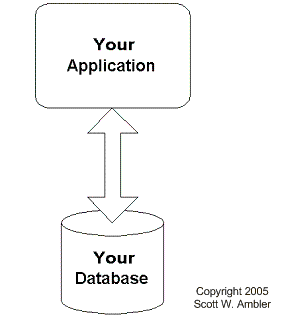
\includegraphics[width=.3\textwidth]{img/dataRefactoringBestCase.png}
		\caption{Baixo Acoplamento}
		\label{figura:1}
	\end{figure}
	
	A Figura~\ref{figura:1} demonstra um cenário \textbf{Single-Database Application} que é bem simplificado, onde a aplicação de uma refatoração exigirá um esforço menor do que a Figura~\ref{figura:2} onde o \textbf{Multi-Application Database} é considerado o pior caso exigindo muito planejamento e cuidado devido a dependência de inúmeras aplicações.

	\begin{figure}[ht]
		\centering
		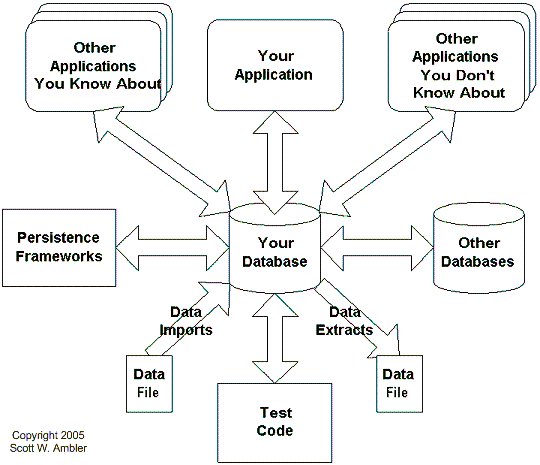
\includegraphics[width=.5\textwidth]{img/dataRefactoringWorstCase.png}
		\caption{Alto Acoplamento}
		\label{figura:2}
	\end{figure}

	
\subsubsection{Processo de refatoração}
	Um processo é um conjunto organizado de atividades com um objetivo em comum. Executar um \textit{database refactoring} em um cenário \textit{Single-Database Application} ou \textit{Multi-Application Database} requer um processo (figura~\ref{figura:3}), por mais simples que seja. A grande diferença na execução em ambos cenários é que no caso do \textit{Multi-Application Database} o período de transição poderá ser mais longo em relação ao \textit{Single-Database Application} \cite{Ambler:RefactoringDatabases}.

	Conforme já citado um \textit{database refactoring} não é uma atividade simples então caso seja identificada a real necessidade de refatorar um banco de dados então pode-se usar o seguinte roteiro (processo) como guia:
	\begin{enumerate}
		\item Escolher o refactoring mais apropriado;
		\item Depreciar o esquema original;
		\item Testar antes, durante e após;
		\item Modificar esquema;
		\item Migrar os dados;
		\item Modificar código externo;
		\item Executar testes de regressão;
		\item Versionar seu trabalho;
		\item Anunciar o refactoring.
	\end{enumerate}

	\begin{figure}[ht]
		\centering
		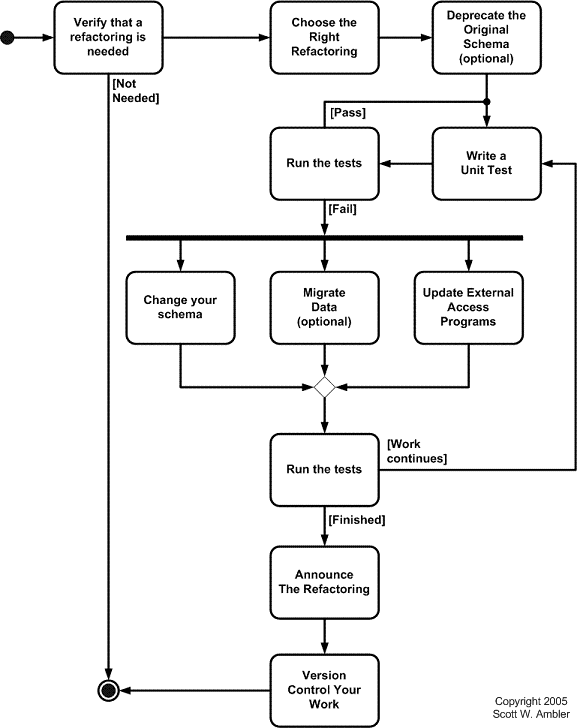
\includegraphics[width=.5\textwidth]{img/databaseRefactoringProcess.png}
		\caption{Processo de Refatoração de Banco de Dados}
		\label{figura:3}
	\end{figure}

	Na Figura~\ref{figura:4} é demonstrado um pequeno ciclo descrevendo um fluxo básico para aplicação de uma refatoração. Deve-se observar com atenção o \textbf{Período de Transição}, que é a fase mais importante, principalmente para cenários \textbf{Multi-Database Application} (Figura 2), onde é importante ter em mente que não geralmente é inviável aplicar a refatoração e \textit{deploy} em ambiente de produção de todas as aplicações ao mesmo tempo. 

	\begin{figure}[ht]
		\centering
		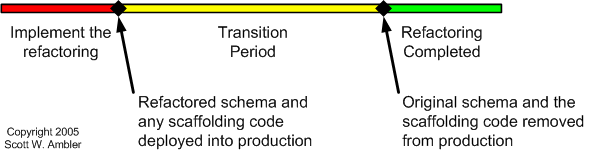
\includegraphics[width=.5\textwidth]{img/databaseRefactoringLifecycle.png}
		\caption{Ciclo de Vida de uma Refatoração de Banco de Dados}
		\label{figura:4}
	\end{figure}

	Dificilmente consegue-se alterar todas as aplicações ao mesmo tempo, principalmente se existir dependência de fornecedores externos, então você será necessário suportar o esquema original e o esquema resultante ao mesmo tempo, para somente quando todas aplicações estiverem suportando apenas o esquema resultante, ou novo esquema, será possível depreciar antigo esquema e assim finalizar este período.

\subsubsection{Estratégias de \textit{Database Refactoring}}
	Existem alguns pontos a considerar como estratégias para adoção de um \textit{database refactoring}:
	\begin{itemize}
		\item Pequenas mudanças são mais fáceis de aplicar;
		\item Identifique unicamente cada refactoring;
		\item Implemente uma grande mudança realizando várias pequenas mudanças;
		\item Tenha uma tabela de configuração/versionamento do seu banco de dados;
		\item Priorize \textit{triggers} ao invés de \text{views} ou sincronizações em lote;
		\item Escolha um período de transição suficiente para realizar as mudanças;
		\item Simplifique sua estratégia de controle de versão de banco de dados;
		\item Simplifique negociações com outros times;
		\item Encapsule acesso ao banco de dados;
		\item Habilite-se a montar facilmente um ambiente de banco de dados;
		\item Não duplique SQL;
		\item Coloque os ativos de banco de dados sobre controle de mudanças;
		\item Seja cuidadoso com políticas.
	\end{itemize}

	Os items acima mostram apenas algumas sugestões, em forma de \textbf{lições aprendidas}, de algumas estratégias que podem ser consideradas quando existir a necessidade de realizar uma refatoração. Para apoiar essas estratégias existe um catálogo que descrevem diversos tipos de refatorações em bancos de dados e exemplos de uso que serão apresentadas no próximo tópico deste trabalho.

\subsubsection{Catálogo de \textit{Database Refactoring}}
	Este catálogo é dividido em algumas categorias:

	\begin{enumerate}
		\item \textit{Structural}: são mudanças na estrutura do banco de dados (tabelas, colunas, visões, etc).
		\item \textit{Data Quality}: são mudanças que melhoram a qualidade das informações contidas em um banco de dados.
		\item \textit{Referential Integrity}: são mudanças que asseguram que uma linha referenciada exista em outra relação e/ou assegura que uma linha que não é mais necessária seja removida apropriadamente.
		\item \textit{Architectural}: são mudanças que melhoram a maneira que programas externos interagem com a base de dados.
		\item \textit{Method}: são mudanças que melhoram a qualidade de uma Procedure um Função.
		\item \textit{Transformations}: mudanças que alteram a semântica do esquema do banco pela adição de novas funcionalidades.
	\end{enumerate}


\subsection{\textit{Database Smells}}
	O autor \cite{Fowler:Refatoracao} introduziu o conceito \textit{code smell} que é uma categoria de problemas recorrentes no código fonte que indica a necessidade de refatoração. De forma similar existem problemas recorrentes em bancos de dados que também indicam a necessidade de sua refatoração \cite{Ambler:RefactoringDatabases}. Seguem alguns exemplos de \textit{smells}:
	\begin{itemize}
		\item \textit{Multipurpose column}: se uma coluna for utilizada para vários fins, é provável que existe um código extra para garantir que a mesma seja usada corretamente e, muitas vezes, verificando valores de uma ou mais colunas.
		\item \textit{Multipurpose table}: quando uma tabela é utilizada para armazenar vários tipos de entidades provavelmente existe uma falha de projeto.
		\item \textit{Redundant data}: é um sério problema em bancos de dados, porque quando o dado é armazenado em vários locais existe alto risco de ocorrer inconsistências.
		\item \textit{Tables with too many columns}: quando uma tabela tem muitas colunas é indicativo de falta de coesão, pois está armazenando dados de várias entidades.
		\item \textit{Tables with too many rows}: tabelas muito grandes podem acarretar problemas de performance. O custo (memória e tempo) para buscar ou atualizar dados em uma tabela varia de acordo com o número de linhas que a mesma possui.
		\item \textit{"Smart" columns}: coluna que armazena informações de mais de um contexto (concatenação de informações).
	\end{itemize}



%\Section{Cronograma de desenvolvimento}\label{sec:cronograma}

%A Tabela \ref{tab:cronograma1} apresenta o cronograma de desenvolvimento do trabalho conforme a numeração das atividades abaixo:
%\begin{enumerate}
%	\item Estudo sobre \textit{database refactoring} e \textit{database smells};
%	\item Montagem dos cenários de teste utilizando os bancos de dados fornecidos por terceiros;
%	\item Estudo sobre taxonomia;
%	\item Realização dos experimentos para identificação de \textit{smells} e aplicação de \textit{refactorings};
%	\item Coleta dos resultados dos experimentos para definição de uma taxonomia e compor um catálogo de \textit{smells} e \textit{refactorings};
%	\item Redação do artigo;
%	\item Submissão do artigo para a banca;
%\end{enumerate}

%\begin{table}[h]
%	\begin{center}
%		\caption{Cronograma de atividades para o trabalho. \label{tab:cronograma1}}
%		\begin{tabular}{|c|c|c|c|c|c|c|}
%			\hline			
%			 \bf Atividade & \bf Jul/2014 & \bf Ago/2014 & \bf Set/2014 & \bf Out/2014 & \bf Nov/2014 & \bf Dez/2014  \\	\hline \hline
%					 1 & x & x & x &   &   &   \\ \hline
%					 2 & x & x &   &   &   &   \\ \hline
%					 3 & x & x & x &   &   &   \\ \hline
%					 4 &   & x & x & x & x &   \\ \hline
%					 5 &   & x & x & x & x &   \\ \hline
%					 6 &   &   & x & x & x &   \\ \hline
%					 7 &   &   &   &   & x &   \\ \hline
%		\end{tabular}
%	\end{center}		
%\end{table}

\Section{Considerações finais}\label{sec:consideracoes}

	Deve-se levar em consideração que apesar destas técnicas serem direcionadas para refatoração, ou seja, mudar estrutura sem mudar sua semântica, as mesmas podem e devem ser utilizadas para evolução da sua aplicação, ou seja, se existe a necessidade de construir uma nova funcionalidade em uma aplicação que está em produção, poderão ser utilizadas as práticas apresentadas neste trabalho para evoluir a estrutura de um banco de dado de forma mais consistente e segura.

	Baseado no que foi apresentado então podemos tentar responder a pergunta \textbf{"Por quê Refatorar?"}:

	\begin{itemize}
		\item aceitar mudança de escopo;
		\item fornecer feedback rápido;
		\item melhoria contínua;
		\item aumentar simplicidade para facilitar entendimento;
		\item tornar os modelos mais próximos do mundo real;
		\item termos modelos simples para facilitar:
		\begin{itemize}
			\item manutenção e
			\item evolução da aplicação
		\end{itemize}
	\end{itemize}

	E para refatorar é necessário conhecimento, disciplina, simplicidade, bom senso e persistência, sem contar no ponto fundamental que é organização.



%\clearpage
\renewcommand\refname{Referências}

\bibliographystyle{cbic2011}
\bibliography{referencias}
\end{document}
